\section{Numerical Results}
\label{sec:numres}
With the mathematical model now fully established, the implementation of this model is documented in Section \ref{subsec:impl}. From here Sections \ref{subsec:vv} verifies the model against approximate plate capacitances modeled using a random walk approach. Finally, Section \ref{subsec:cs} investigates the convergence of all three formulations to a single numerical value as a function of the asymptotic number of operations required to obtain these capacitance values.

\subsection{Implementation}
\label{subsec:impl} 
For the purposes of this study, only a square plate of side length $l=0.01$m is considered. This plate is broken up into an $n\times n$ grid of square surface elements as this is what all formulations of the system matrix are derived for as found in Section \ref{subsub:mat-form}. In Secton \ref{subsec:vv}, the value of $n$ will range from 10-30 for verification and validation against plate capacitance values found in the literature. These values will be expanded in Section \ref{subsec:cs} to range between 10-100 to model convergence to a single numerical value.

All code for this model was written in Python for its ease of use and plentiful numeric packages such as NumPy and SciPy, both of which were used. The model is constructed in a way to handle system matrix assembly for any number of elements per side and side length for square plates thus making it flexible for this analysis.

\subsection{Verification and Validation}
\label{subsec:vv}
Prior to performing any novel analysis, the model first needs to be validated against theory. In 2004, H. J. Wintle used Monte Carlo methods to place a bound on dimensionless capacitance of square plates \cite{randomwalk}. Their models resulted in a dimensionless capacitance $C^*=0.36\pm0.01$ for square plates defined as
\begin{align}
	C^*=\frac{C}{4\pi\epsilon_0l}
\end{align}
where $C$ is the true capacitance value and $l$ is the side length of the plate in meters \cite{randomwalk}. Using a side length of $l=0.01$m, this bound maps to the capacitance range of 0.389-0.411pF. Thus if for some number of elements per side length, $n$, the model is able to predict values within this range, they are technically valid.

To predict the capacitance of the square plate we, first integrate the charge distribution over all elements which gives the total charge. From basic electrostatics, the capacitance is then determined by dividing the total charge by the arbitrary choice of potential. This mapping and corresponding reduction over all $M$ elements is written succinctly as 
\begin{align}
	C=\frac{S}{\Phi_0}\sum_{m=0}^{M-1}\rho_{s}^{(m)}
\end{align}
where $S$ is the surface area of a single square element, and $\rho_{s}^{(m)}$ is the surface charge density associated with the $m^{th}$ element.

Applying this map-reduce operation to the surface charge distributions obtained from solving (\ref{eq:linsys}) results in the following capacitance values as found in Table 1.

\begin{table}[h!]
	\centering
\begin{tabular}{ |p{2cm}||p{1cm}|p{1cm}|p{1cm}|}
	\multicolumn{4}{c}{Table 1: Predicted Capacitances by Method} \\
	\hline
	Method & $10\times10$ & $20\times20$ & $30\times30$ \\
	\hline
	Circular Element Approximation   & 0.397pF &0.403pF & 0.405pF\\
	\hline
	Exact Square Elements& 0.394pF& 0.401pF & 0.403pF\\
	\hline
	Subdomain Collocation&0.399pF & 0.403pF & 0.405pF \\
	\hline
   \end{tabular}
   \label{tab:capvals}
\end{table}

As seen in Table 1, the capacitances of all system matrix formulations for all grid resolutions technically converge to the Monte Carlo solution reported in \cite{randomwalk}. In general, the circular element approximation is generally very similar to the subdomain collocation method while the exact square element solution trails slightly behind these methods. Based on this it is assumed that the circular element approximation over estimates the charge density slightly which results in it behaving similarly to subdomain collocation using an entirely different testing function. Further discussion on convergence will be included in Section \ref{subsec:cs}. 

With the capacitance models validated for all mesh resolutions and system matrix formulations, the charge distributions are now analyzed to ensure correctness of the overall distribution and not just total charge. With this, surface charge distributions for $10\times10$, $20\times20$, and $30\times30$ grids using subdomain collocation are found in Fig. \ref{fig:charge_d}. 

As shown in Fig. \ref{fig:charge_d}, the charge distribution for all grid resolutions is focussed on the edges of the plate and is most intense in the corners. This can be understood from basic electrostatic theory as like charges repel. Thus, charges will most likely accumulate in locations with fewer "neighboring charges", namely the corners and edges of the plate. Also seen in Fig. \ref{fig:charge_d}, the final "form" of the charge distribution is reached by the $20\times 20$ grid. This metric is rather subjective and is based on a pseudocolor map thus will not be expanded further. In addition to this, the choice of using subdomain collocation is entirely arbitrary. This formulation was chosen as it was deemed the most accurate due to its use of a first order pulse testing function. Distributions for the circular element approximation and exact square element solution looked nearly identical and thus were not included.

\begin{figure}[t!]
	\begin{subfigure}{\linewidth} %\make this subfigure take up 80% of a linewidth
		\centering
		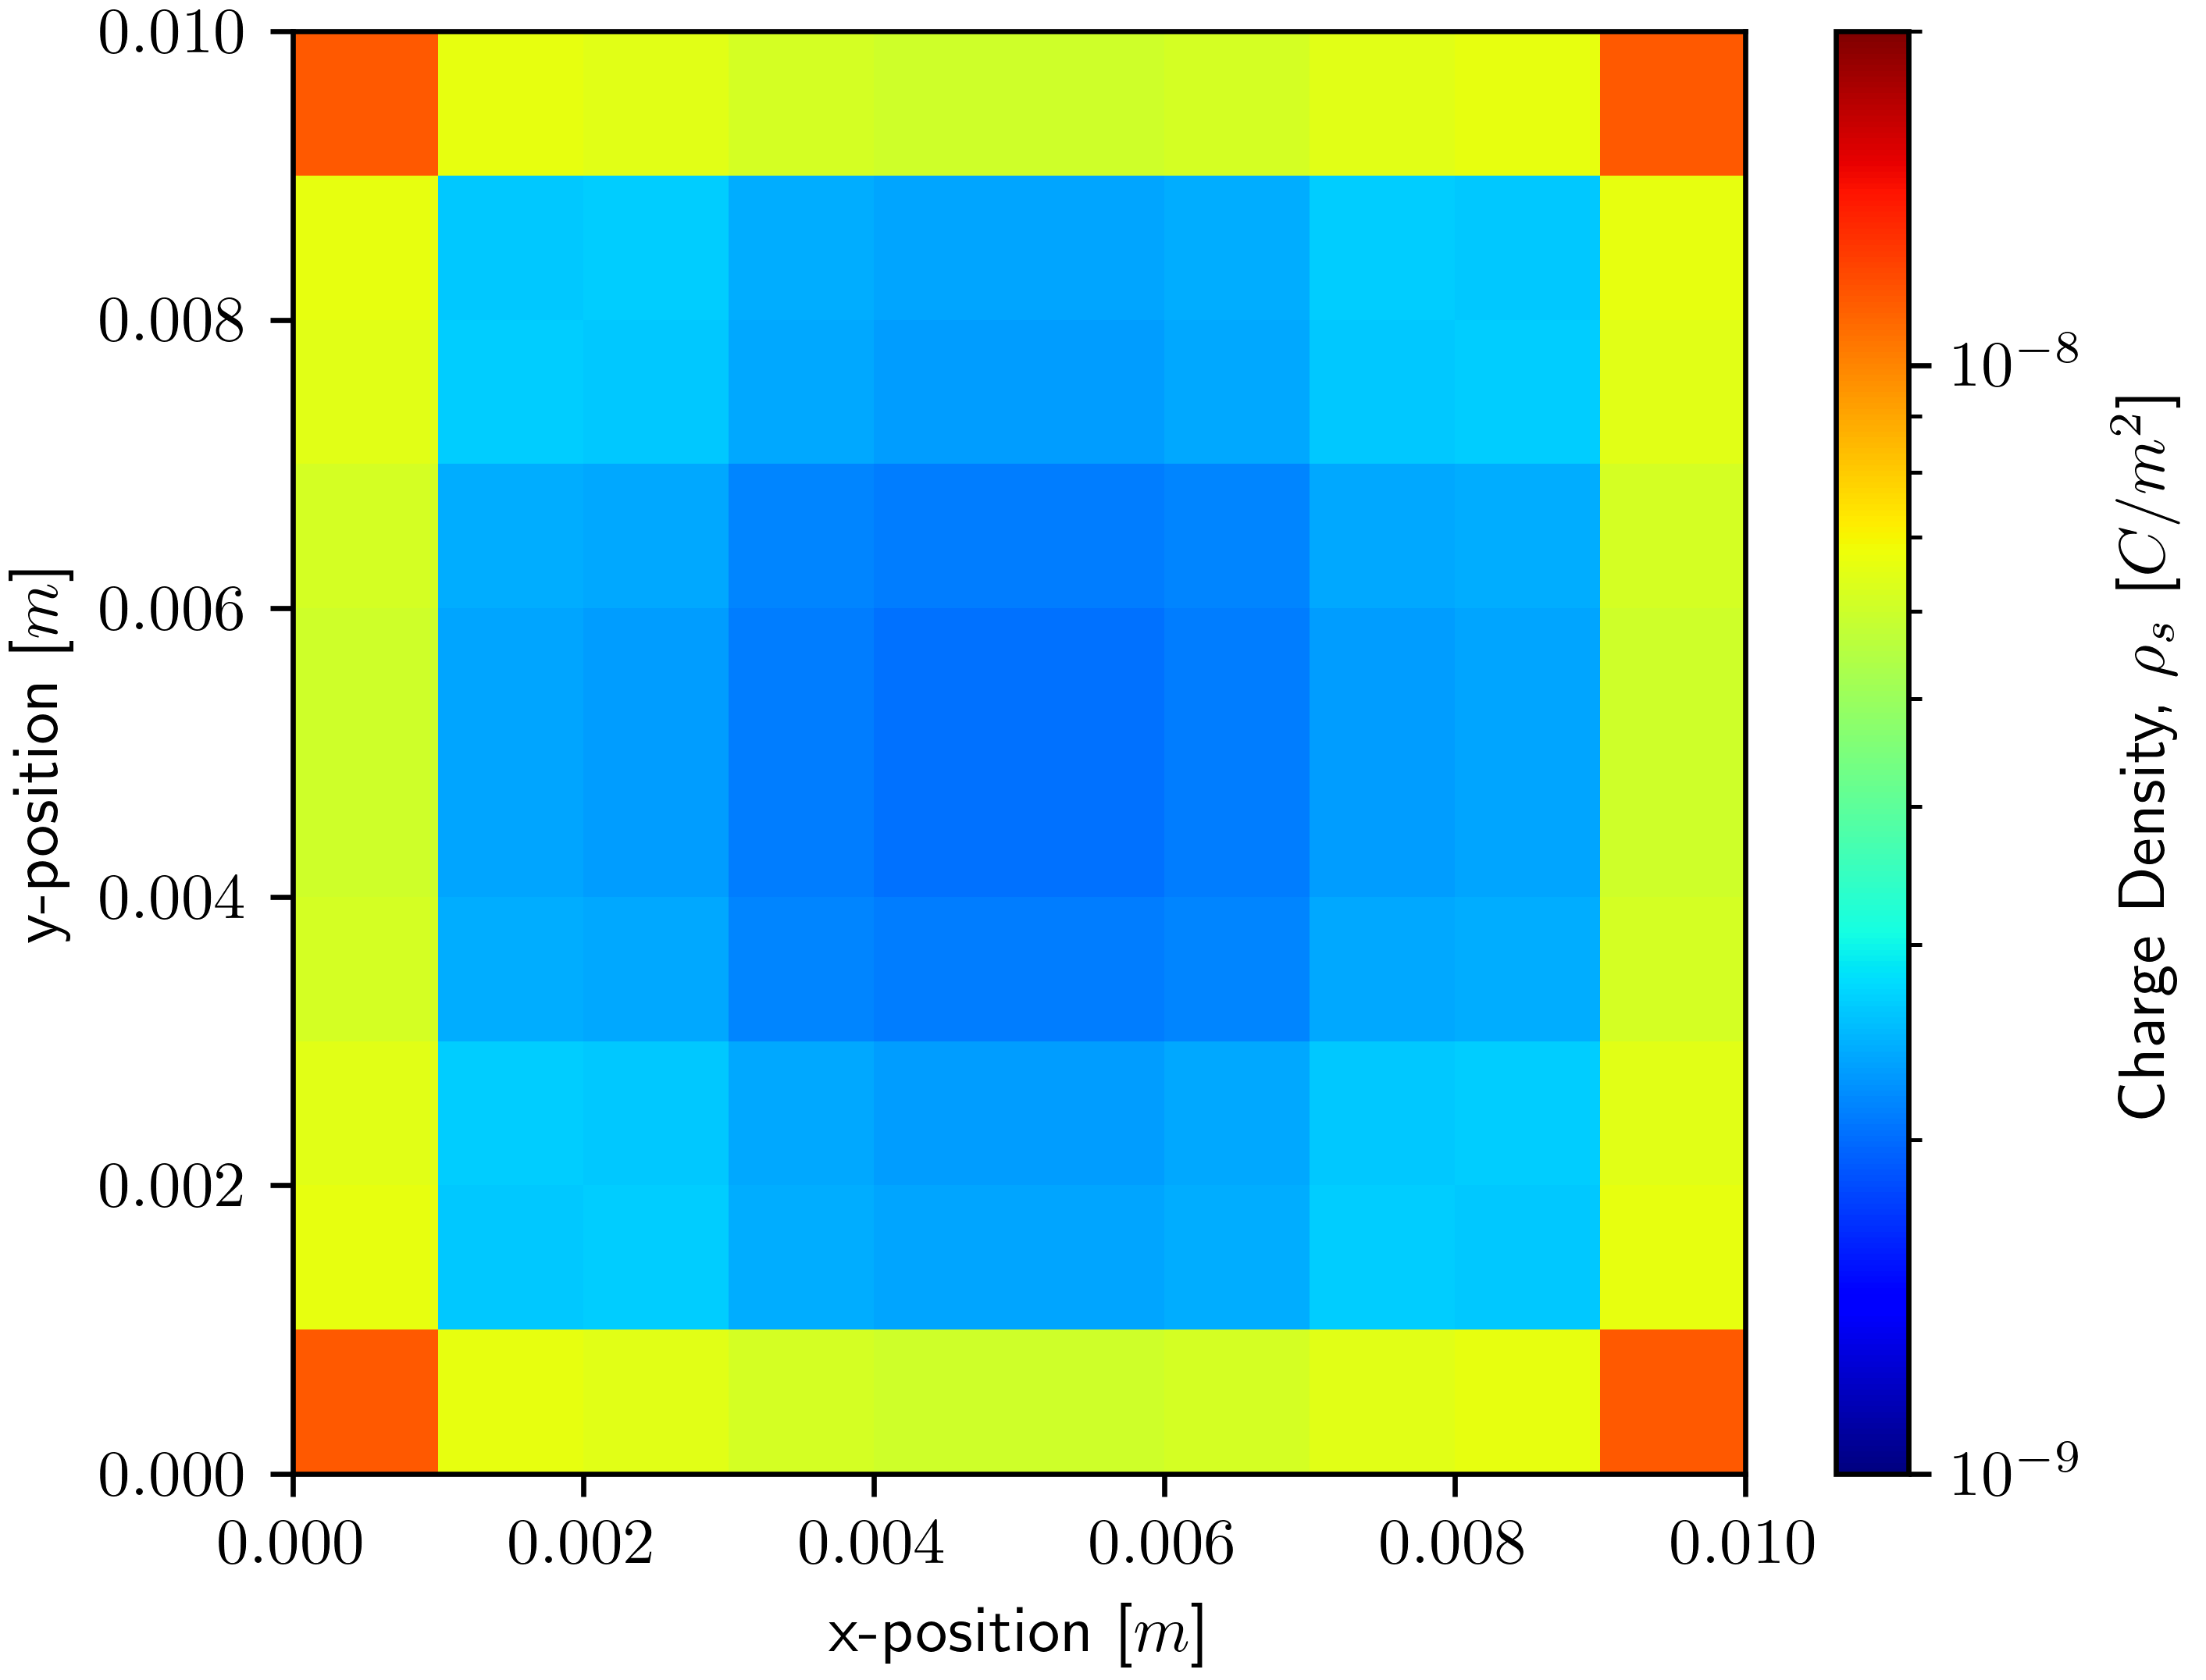
\includegraphics[width=\textwidth]{subd_10.png} %within this subfigure take up the entire textwidth (which was set by the linewidth command above)
		\caption{}
		\label{subfig:d10}
	\end{subfigure}
	\begin{subfigure}{\linewidth}
		\centering
		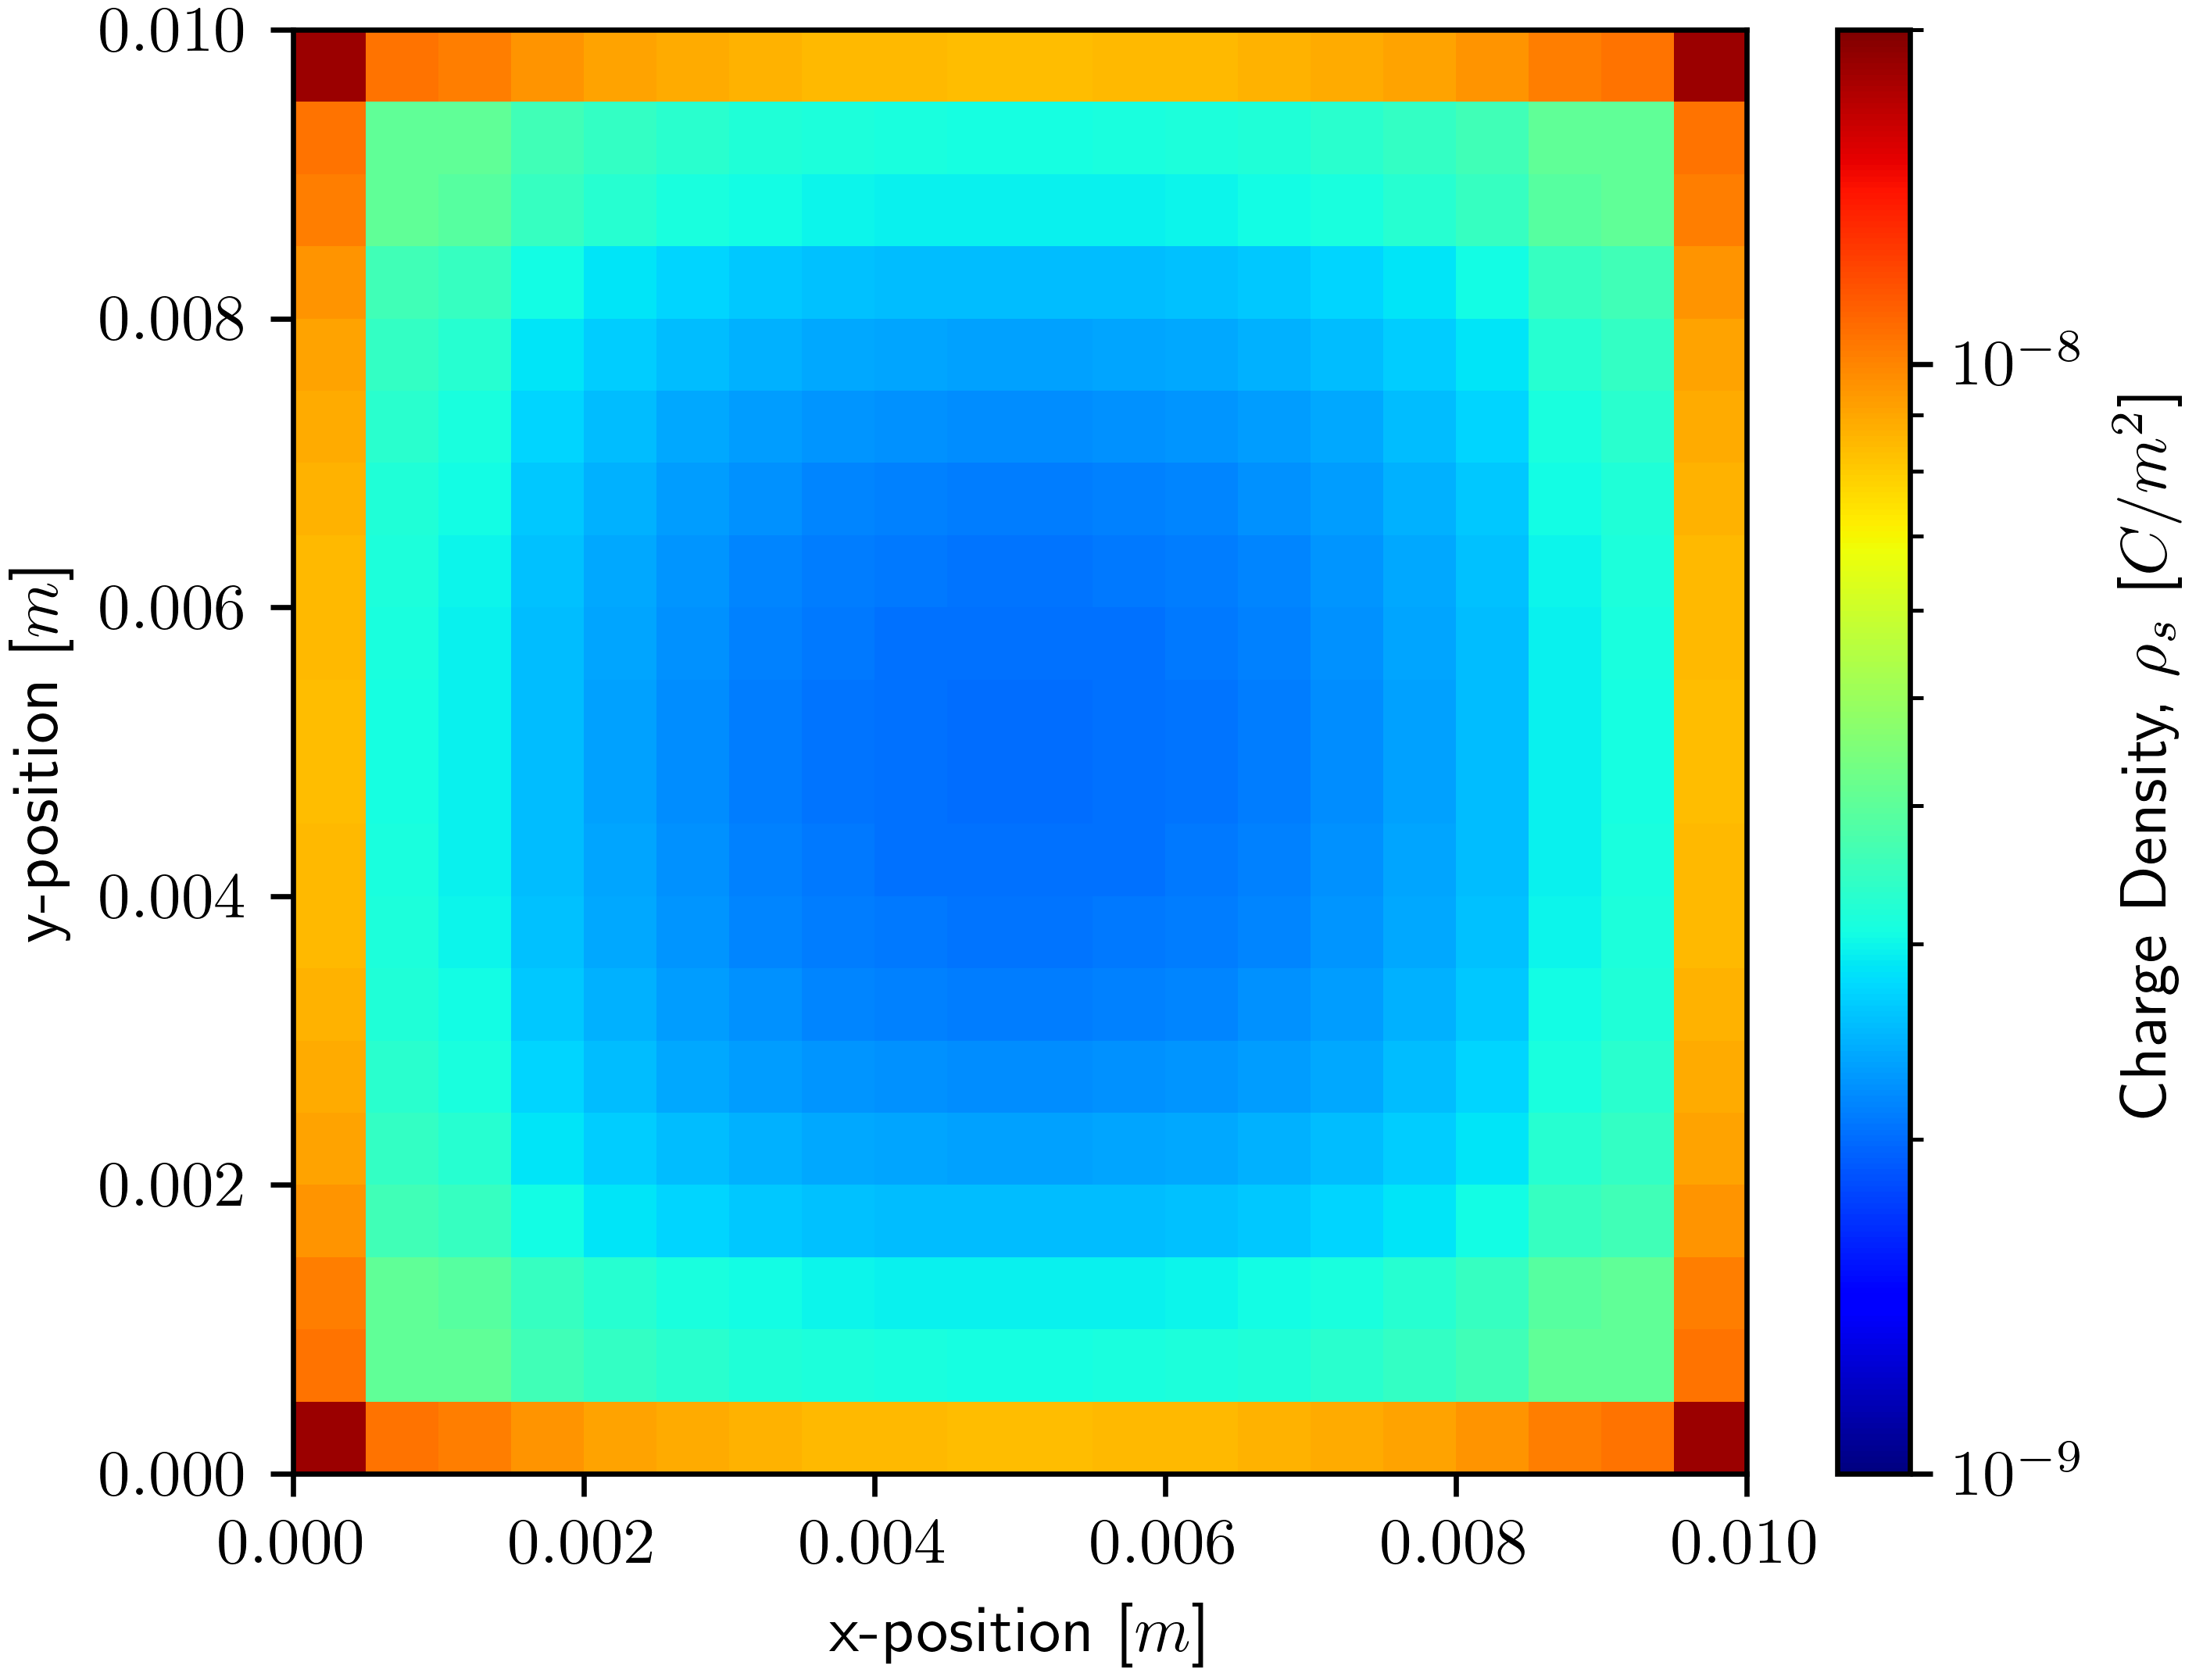
\includegraphics[width=\textwidth]{subd_20.png} %waveport2 is the name of the jpg file within the ./figures folder
		\caption{} %leave the caption blank, but you need the empty caption command for the (b) label to be made
		\label{subfig:d20}
	\end{subfigure}
	\begin{subfigure}{\linewidth}
		\centering
		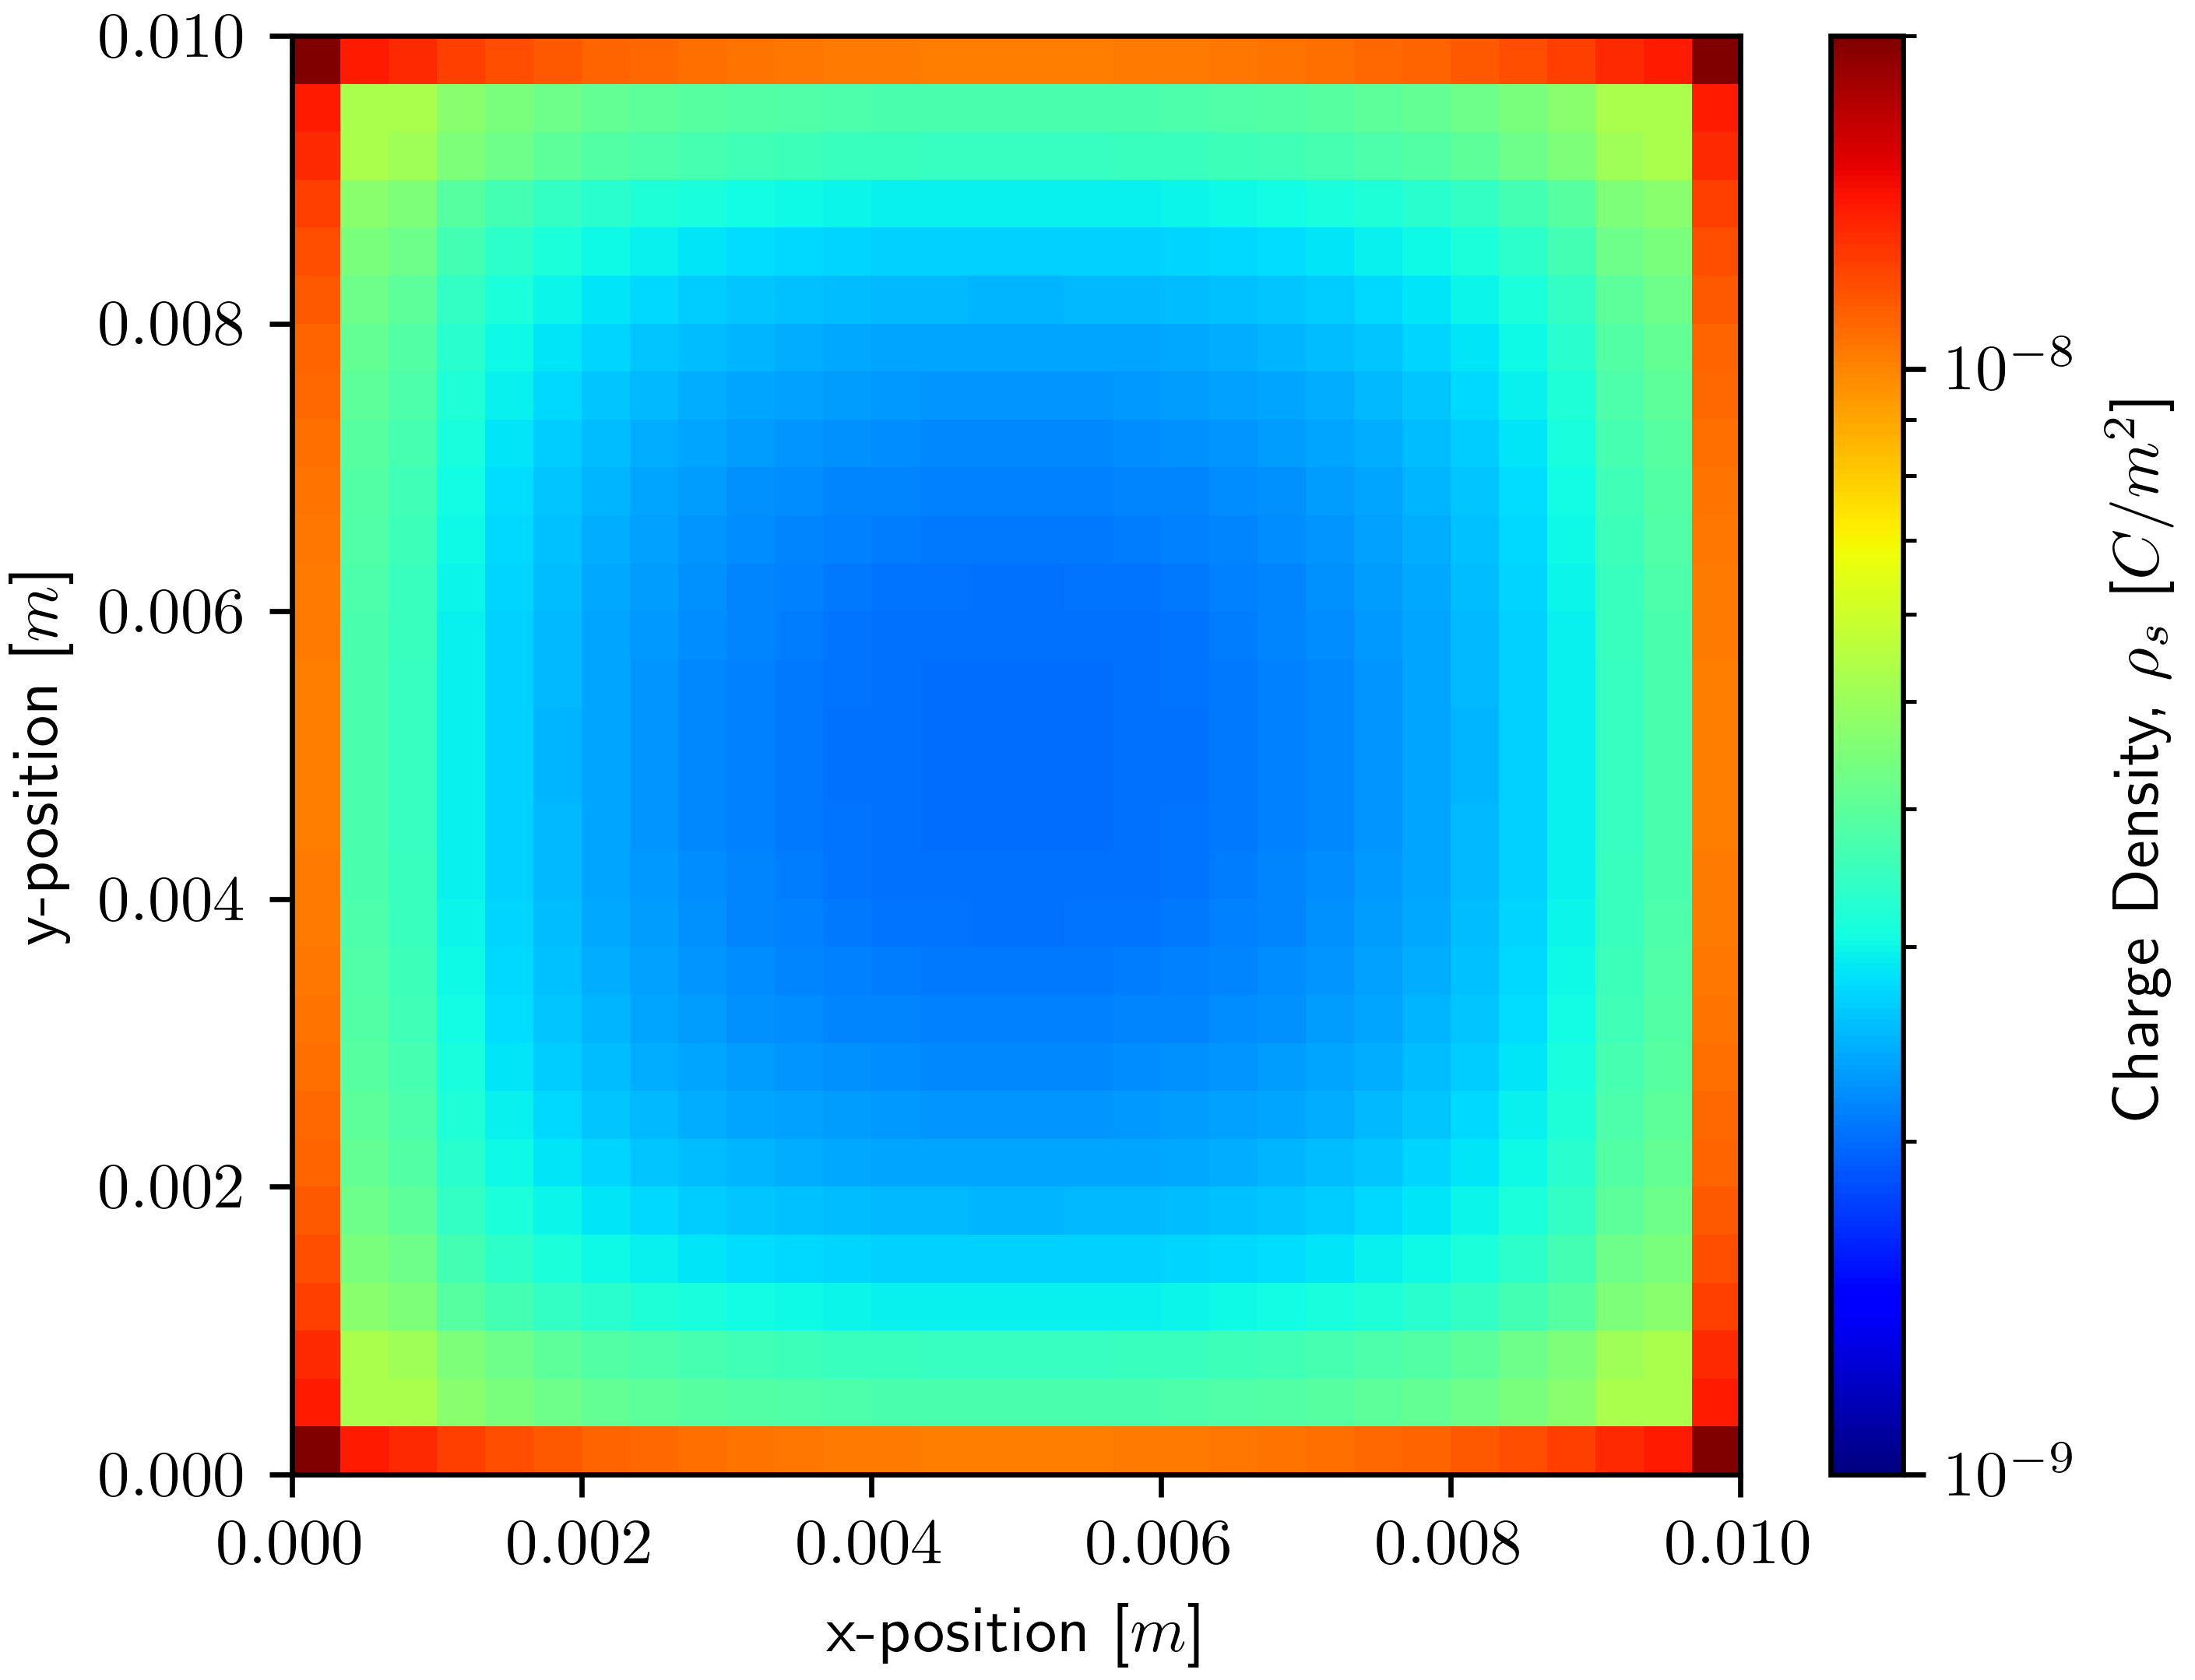
\includegraphics[width=\textwidth]{subd_30.png} %waveport2 is the name of the jpg file within the ./figures folder
		\caption{} %leave the caption blank, but you need the empty caption command for the (b) label to be made
		\label{subfig:d30}
	\end{subfigure}
	\caption{Surface Charge Density ($\rho_s$) distributions using Subdomain Collocation for mesh resolutions of (a) $10\times10$ (b) $20\times20$ and (c) $30\times30$.}
	\label{fig:charge_d}
\end{figure}


\subsection{Convergence Study}
\label{subsec:cs}
With the model successfully validated, it is now important to compare the convergence rates between these methodologies. As discussed in Section \ref{subsec:vv}, the predicted capacitances of all three formulations and grid resolutions technically converged to capacitance ranges reported in the literature; however, these methods did not necessarily converge to a single value. This begs the following question: what numerical value, if any, do these methods converge to? To this end, a convergence study was performed extending the maximum resolution to a $100\times 100$, sweeping over intermediate resolutions. This maximum resolution was chosen as it was the largest matrix the model, as described, could resolve in a `reasonable' amount of time. Limitations of the model will be discussed further in Section \ref{sec:conclusion}. Results of this sweep can be found in Fig \ref{fig:convergence} as a function of the asymptotic number of operations required to obtain said solutions which is $O(n^3)$ for dense matrices. 

\begin{figure}[h!]  
	\centering
	%the command within the [] sets the width of the figure, stability-condition is the jpg name
	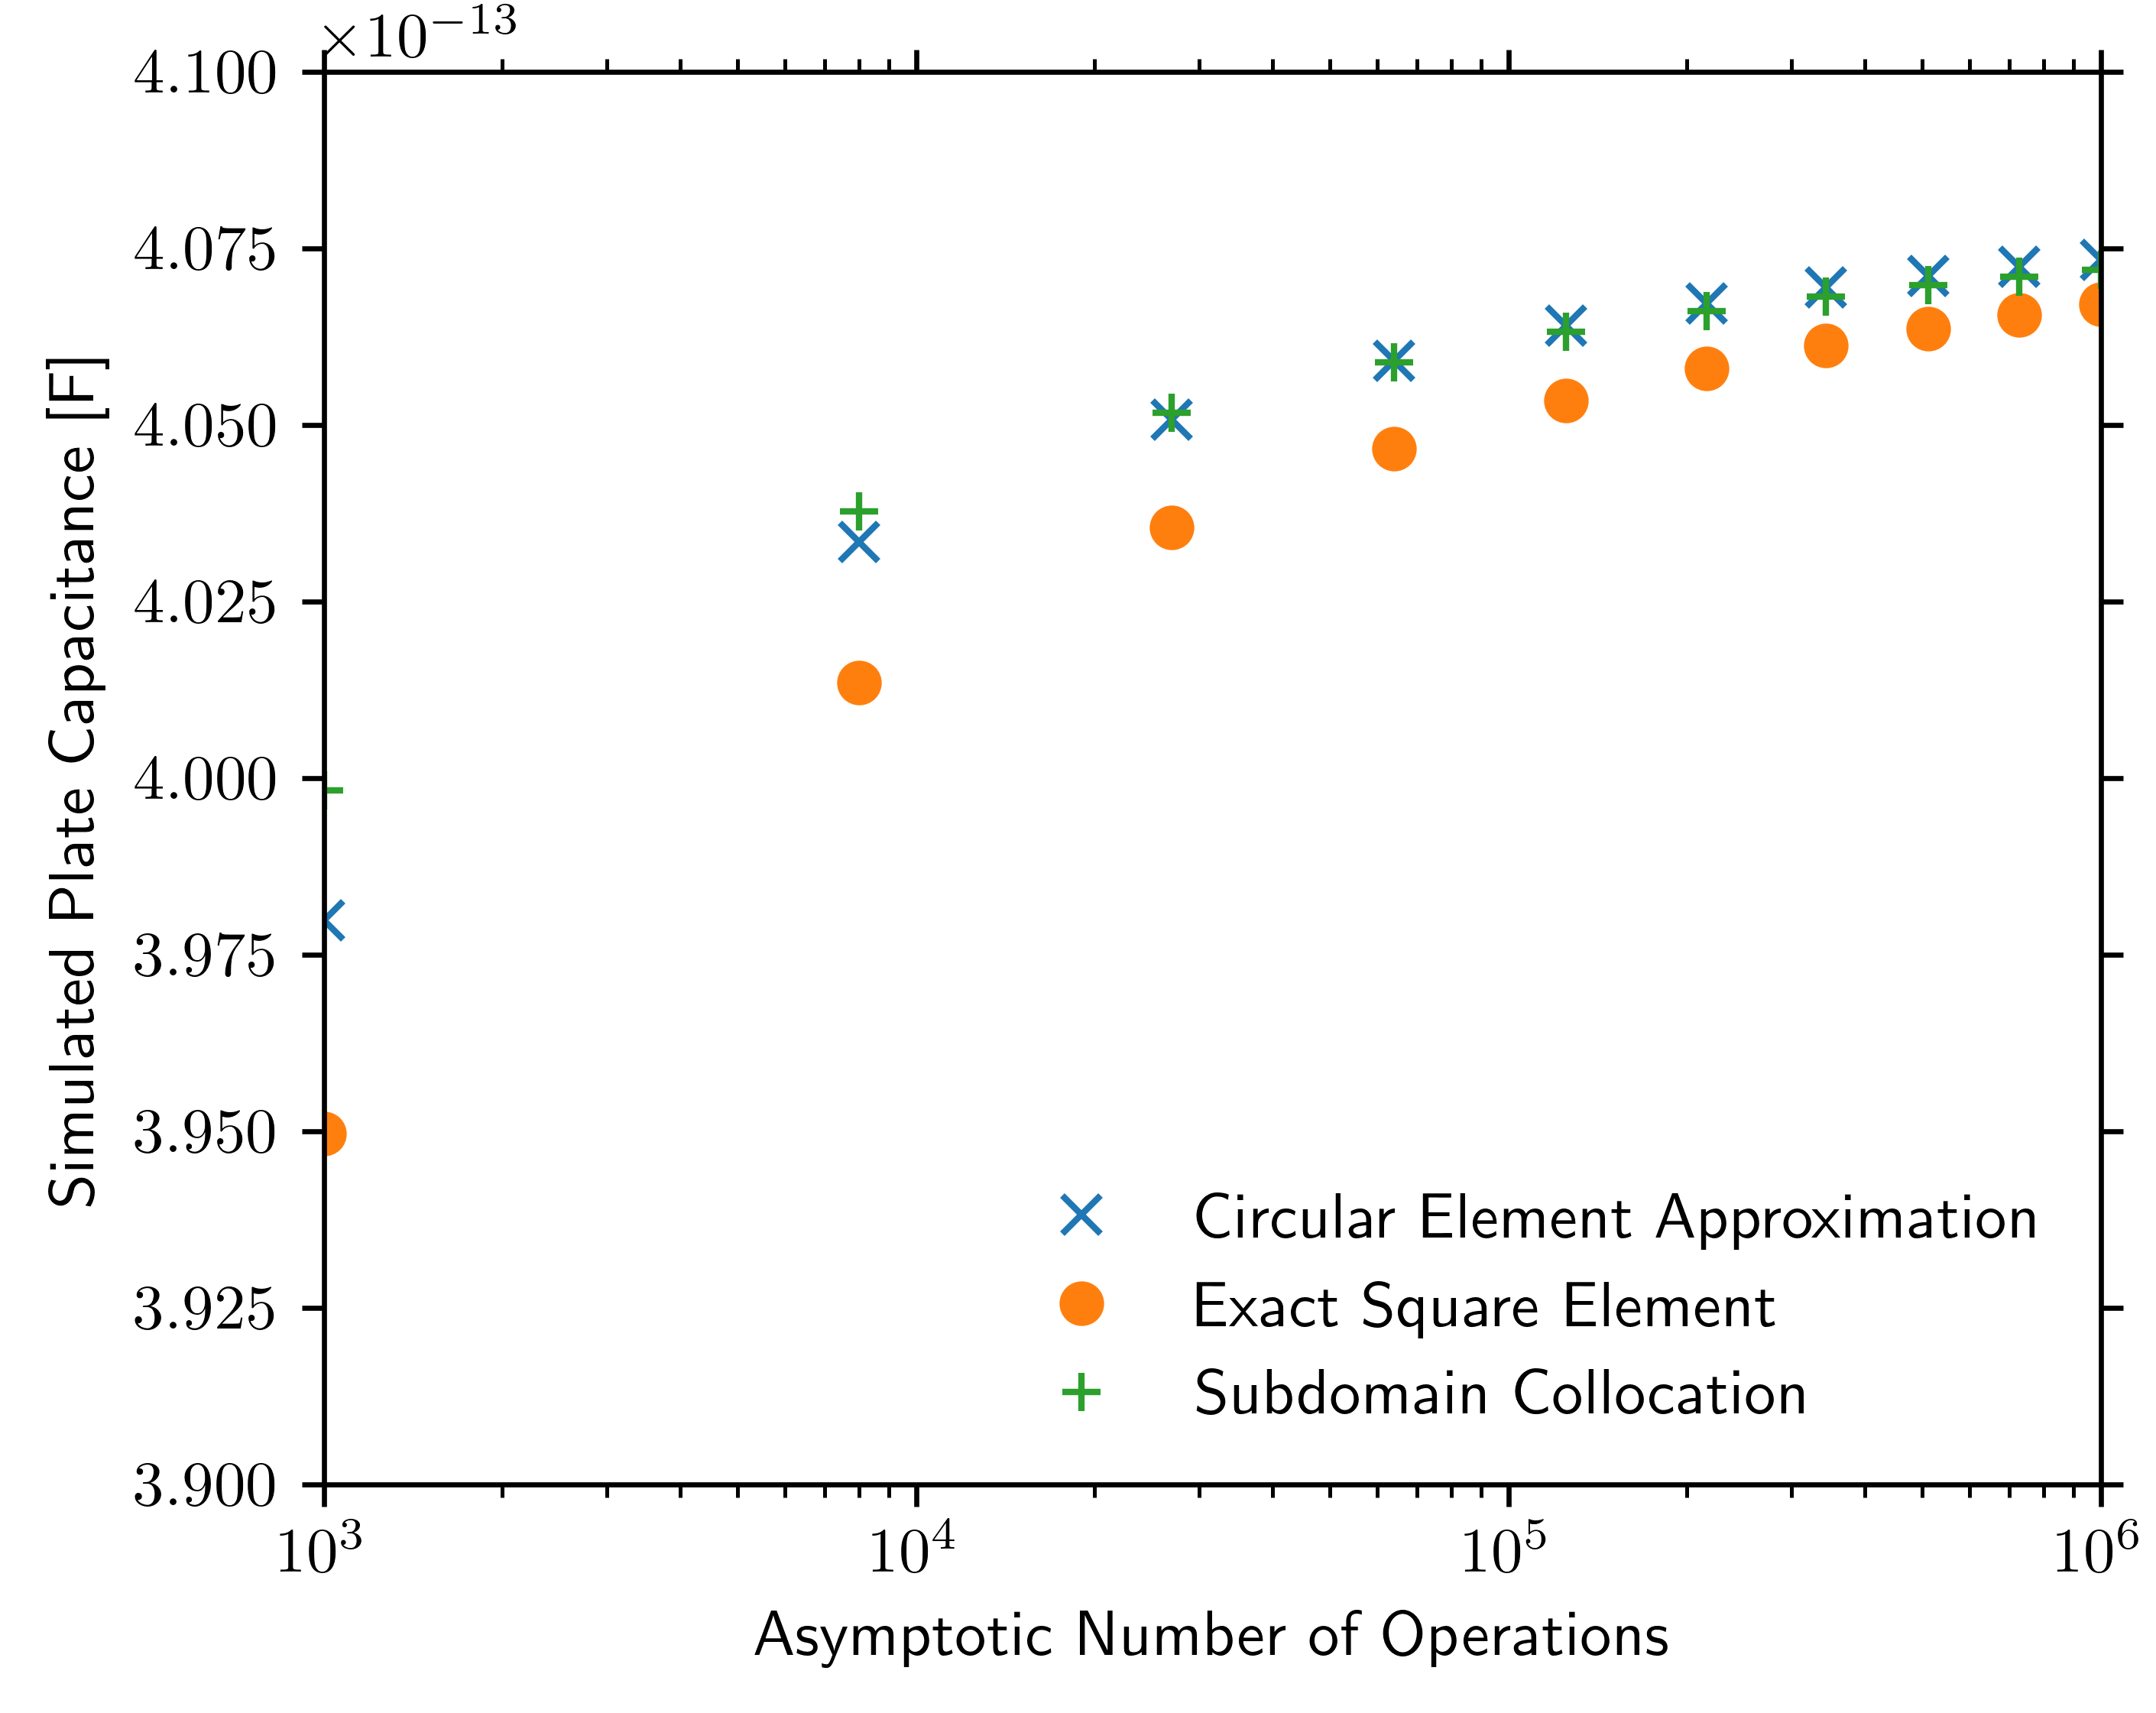
\includegraphics[width=\linewidth]{conv.png} 
	\caption{Convergence Study of All Three System Matrix Formulations Over a Wide Range of Grid Resolutions}
	\label{fig:convergence}
\end{figure}

As seen in Fig. \ref{fig:convergence}, as the grid resolution, and corresponding number of asymptotic operations increases, all three formulations converge on a capacitance of approximately $0.4075$pF. A simple percent difference analysis reveals that these methods produce the same value within $0.1\%$ of each other for $n\geq30$. This low percent difference results in the circular approximation of square surface elements being the ideal choice for this problem for its overall simplicity and rapid assembly process for matrices on the order of those studied here. This fact would change however if the matrices were far larger. For example, there exist scalable and memory efficient algorithms for solving dense symmetric matrices as those found in subdomain collocation far quicker than dense unsymmetrical matrices found in both of the methodologies using the delta function as a testing function\cite{densesym}. Thus for solving larger, more complex systems, the subdomain collocation method becomes the optimal choice.